\documentclass{standalone}
\usepackage{tikz}
\usepackage{ctex,siunitx}
\setCJKmainfont{Noto Serif CJK SC}
\usepackage{tkz-euclide}
\usepackage{amsmath}
\usetikzlibrary{patterns, calc,3d}
\usetikzlibrary {decorations.pathmorphing,decorations.pathreplacing,decorations.shapes}
\tikzset{label style/.append style={font=\small}}
\begin{document}
\small
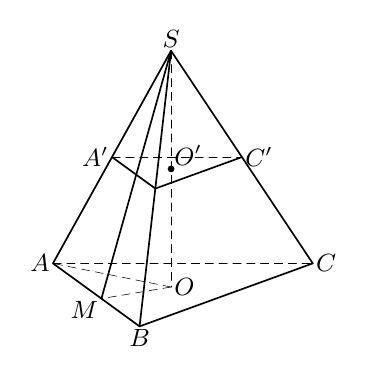
\begin{tikzpicture}[>=latex,scale=1.0,inner sep=1pt]
  \tkzDefPoints{0/0/O,0/3/S,-1.5/0.3/A,1.8/0.3/C,-0.4/-0.5/B}
  \tkzInterLL(C,O)(A,B)\tkzGetPoint{M}
  \tkzDefPointOnLine[pos=0.5](S,O)\tkzGetPoint{O'}
  \tkzDefPointOnLine[pos=0.5](S,A)\tkzGetPoint{A'}
  \tkzDefPointOnLine[pos=0.5](S,B)\tkzGetPoint{B'}
  \tkzDefPointOnLine[pos=0.5](S,C)\tkzGetPoint{C'}
  \tkzDrawPolygon[semithick](A,B,C,S);
  \tkzDrawPoints[fill=black](O')
  \tkzDrawSegments[densely dashed](S,O O,M A,C O,A A',C')
  \tkzDrawSegments[semithick](S,M S,B A',B' B',C')
  \tkzLabelPoints[left](A,A')
  \tkzLabelPoints[below left](M)
  \tkzLabelPoints[above](S)
  \tkzLabelPoints[above right](O')
  \tkzLabelPoints(B)
  \tkzLabelPoints[right](C,C',O)
\end{tikzpicture}
\end{document}